%------------------------------------------------------------------------------
% CV in Latex
% Author : Charles Rambo
% Based off of: https://github.com/sb2nov/resume and Jake's Resume on Overleaf
% Most recently updated version may be found at https://github.com/fizixmastr 
% License : MIT
%------------------------------------------------------------------------------

\documentclass[A4,11pt]{article}
%\documentclass[letterpaper,11pt]{article} %For use in US
\usepackage{latexsym}
\usepackage[empty]{fullpage}
\usepackage{titlesec}
\usepackage{marvosym}
\usepackage[usenames,dvipsnames]{color}
\usepackage{verbatim}
\usepackage{enumitem}
\usepackage[hidelinks]{hyperref}
\usepackage[english]{babel}
\usepackage{tabularx}
\usepackage{tikz}
\input{glyphtounicode}
\usepackage{latexsym}
\usepackage[empty]{fullpage}
\usepackage{titlesec}
\usepackage{marvosym}
\usepackage[usenames,dvipsnames]{color}
\usepackage{verbatim}
\usepackage{enumitem}
\usepackage[hidelinks]{hyperref}
\usepackage{fancyhdr}
\usepackage[english]{babel}
\usepackage{tabularx}

% my added package for map marker
\usepackage{fontawesome}


\input{glyphtounicode}



%-----FONT OPTIONS-------------------------------------------------------------
\begin{comment}
The font of the document will impact not just how readable it is, but how it is
perceived. In the "The Craft of Scientific Writing" by Michael Alley, shares a
common fonts for publication as well as their use. I have chosen to use
Palatino for its legibility, some others are given below. There is far too much
about typography to discus here. Note: serif fonts have short projecting
strokes, sans-serif fonts are sans (without) these strokes.
\end{comment}


% serif
 \usepackage{palatino}

\addtolength{\oddsidemargin}{-1cm}
\addtolength{\evensidemargin}{-1cm}
\addtolength{\textwidth}{2cm}
\addtolength{\topmargin}{-1cm}
\addtolength{\textheight}{2cm}



\urlstyle{same}

\raggedbottom
\raggedright
\setlength{\tabcolsep}{0cm}

\titleformat{\section}{
  \vspace{-4pt}\scshape\raggedright\large
}{}{0em}{}[\color{black}\titlerule \vspace{-5pt}]

\pdfgentounicode=1

\newcommand{\CVItem}[1]{
  \item\small{
    {#1 \vspace{-2pt}}
  }
}

\newcommand{\CVSubheading}[4]{
  \vspace{-2pt}\item
    \begin{tabular*}{0.97\textwidth}[t]{l@{\extracolsep{\fill}}r}
      \textbf{#1} & #2 \\
      \small#3 & \small #4 \\
    \end{tabular*}\vspace{-7pt}
}
\newcommand{\medi}[3]{
  \vspace{-2pt}\item
    \begin{tabular*}{0.97\textwidth}[t]{l@{\extracolsep{\fill}}r}
      \textbf{#2} & #1 \\
      \small#3 \\
    \end{tabular*}\vspace{-7pt}
}
\newcommand{\CVSubheadingshort}[2]{
  \vspace{-2pt}\item
    \begin{tabular*}{0.97\textwidth}[t]{l@{\extracolsep{\fill}}r}
      \textbf{#1} & #2 \\
    \end{tabular*}\vspace{-7pt}
}
\newcommand{\CVSubSubheading}[2]{
    \item
    \begin{tabular*}{0.97\textwidth}{l@{\extracolsep{\fill}}r}
      \text{\small#1} & \text{\small #2} \\
    \end{tabular*}\vspace{-7pt}
}

\newcommand{\CVSubItem}[1]{\CVItem{#1}\vspace{-4pt}}

\renewcommand\labelitemii{$\vcenter{\hbox{\tiny$\bullet$}}$}

\newcommand{\CVSubHeadingListStart}{\begin{itemize}[leftmargin=0.5cm, label={}]}
\newcommand{\CVSubHeadingListEnd}{\end{itemize}}
\newcommand{\CVItemListStart}{\begin{itemize}}
\newcommand{\CVItemListEnd}{\end{itemize}\vspace{-5pt}}
\begin{document}

\begin{comment}
\end{comment}

\begin{minipage}[c]{0.05\textwidth}
\-\
\end{minipage}
\begin{minipage}[c]{0.2\textwidth}
\begin{tikzpicture}
    \clip (0,0) circle (1.75cm);
    \node at (0,-.3) {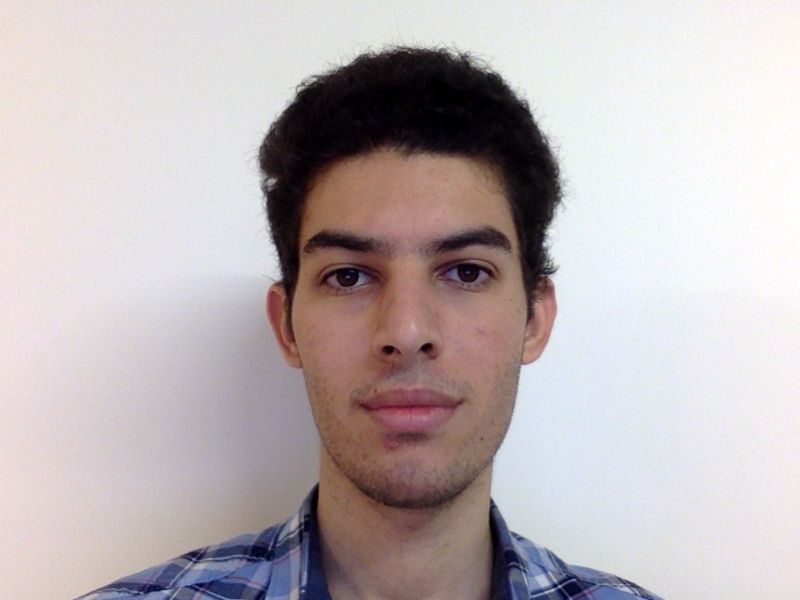
\includegraphics[width = 5cm]{moi}}; 
\end{tikzpicture}
\hfill\vline\hfill
\end{minipage}
\begin{minipage}[c]{0.6\textwidth}
    \textbf{\Huge \scshape{Omar Mohsen}} \\ \vspace{1pt} 
    \small{\faPhone +33 7 81 32 99 93} \\\small{01 Mars 1996 $|$ French $|$ Egyptian}\\
   % \href{mailto:omar.mohsen.fr@gmail.com}{\underline{\faEnvelope\thinspace omar.mohsen.fr@gmail.com}} \\
   \href{mailto:omar.mohsen@imj-prg.fr}{\underline{\faEnvelope\thinspace omar.mohsen@imj-prg.fr}}\\ \href{https://sites.google.com/view/omar-mohsen-webpage/home}{\underline{\faGoogle\thinspace sites.google.com/view/omar-mohsen-webpage/home}} \\
   \href{https://github.com/OmarMohsenGit}{\underline{\faGithub \thinspace github.com/OmarMohsenGit}}
  \end{minipage}

%-----EDUCATION----------------------------------------------------------------
\section{Scientific Career}
  \CVSubHeadingListStart
  \CVSubheading
      {{Professor}}{September 2025 -- Current}
      {\href{https://www.imj-prg.fr/}{\underline{Paris Cité University}}}{France}   
\CVSubheading
      {{Maître de conférence (research/teaching position)}}{September 2021 -- August 2025}
      {Paris-Saclay University}{France}   
    \CVSubheading
      {{Postdoc}}{September 2019 -- August 2021}
      {University of Muenster}{Germany}
        \CVSubheading
      {{ATER (Teaching Position)}}{October 2018 -- August 2019}
      {Sorbonne Paris Cité}  {France}
  \CVSubHeadingListEnd
\section{Education}
  \CVSubHeadingListStart
   \CVSubheading
      {Habilitation}{2025}
      {Defended on 03 February 2025 at Paris-Saclay University}{France}
    \CVSubheading
      {{PhD $|$ \emph{\small{Thesis defended in October 2018 under the direction of \href{https://webusers.imj-prg.fr/~georges.skandalis/}{\underline{G. Skandalis}}}}}}{2015 -- 2018}
      {Sorbonne Paris Cité. More details \href{https://theses.fr/2018USPCC200}{\underline{here}}}{France}
    \CVSubheading
      {{Diploma from ENS}}{2012 -- 2015}
      {École normale supérieure de Paris}{France}
    \CVSubheading
      {Master}{2013 -- 2015}
      {Paris-Saclay University}{France}
  \CVSubHeadingListEnd
  \section{Scientific Distinctions}
\CVSubHeadingListStart
\CVSubheadingshort{\href{https://www.bourbaki.fr/TEXTES/Exp1236-Debord.pdf}{\underline{Bourbaki seminar 1236 on our work by C. Debord}}}{2025}{}{}
\CVSubheadingshort{\href{}{Medal from the faculty of Science Cairo university}}{2024}{}{}
\CVSubheadingshort{\href{https://www.college-de-france.fr/fr/personne/omar-mohsen}{\underline{Prix Peccot from Collège de France}}}{2024}{}{}
   \CVSubheadingshort{\href{https://www.insmi.cnrs.fr/en/cnrsinfo/prix-academie-des-sciences-2024-mathematiques}{\underline{Prix Jacques Herbrand from the french academy of sciences}}}{2024}{}{}
\CVSubHeadingListEnd
 
\section{Grants}
  \CVSubHeadingListStart
  \CVSubheading
{\href{}{RIPEC C3}}{2024-2027}{Research grant}{France}
\CVSubheading
{ANR}{2023}
{\href{https://anr.fr/Project-ANR-23-CE40-0016}{\underline{Part of the ANR team OPART}}}{France}
    \CVSubheading
      {Région Ile de France, FSMP}{2015-2018}
      {PhD Scholarship}{France}
      \CVSubheading
      {Fondation Sciences Mathématiques de Paris (FSMP)}{2013-2015}
      {Master's Scholarship}{France}
       \CVSubheading
      {Fondation Mathématiques Jacques Hadamard (FMJH)}{2012}
      {License Scholarship}{France}
  \CVSubHeadingListEnd
  \section{Supervision}
  \CVSubHeadingListStart
  \CVSubheadingshort{\href{}{Paul Quiñones, Jacques Dubot, Zoé Chantreuil, Traian Demais, Paul Miltgen}}{2025 M1}
  \CVSubheadingshort
{\href{}{Enzo Tanguide}}{2025 M2}
\CVSubheadingshort
{Julie Capron, Oleksii Shulga, Quentin Casella, Enzo Tanguide}{2024 M1}
\CVSubheadingshort
{\href{}{Moudrik Chamoux}}{2024 M2}
    \CVSubheadingshort
      {Anatole Dedecker}{2023 M1}
      \CVSubheadingshort
      {Matiss Brunel, Quentin Giton, Flore le Roux}{2022 L3}

  \CVSubHeadingListEnd
  \section{Scientific Evaluation}
  I was referee for the following journals: Advances in Mathematics, Annales de l'Institut Fourier, Annales Henri Lebesgue, Astérisque, Bulletin des sciences mathématiques, Communications in Partial Differential Equations, Comptes rendus de l'académie des sciences, Crelle journal, Journal of Differential Equations, Journal of Geometric analysis, Journal of Geometry and Physics, Journal of noncommutative geometry, Math. Ann.  , Muenster journal of mathematics, Pacific Journal of Mathematics
  
  \section{Administrative responsibilities}
  \CVSubHeadingListStart
  \CVSubheadingshort
{Member of the Orsay laboratory of mathematics advisory committee}{2023-2025}
  \CVSubHeadingListEnd


  \section{Scientific responsibilities}
 \CVSubHeadingListStart
 \CVSubheading
{ Bernoulli Center for Fundamental Studies }{2025}
{Organization member with F. Nier, S. Shen, T. Lelievre for the program "New trends and applications \\ around generalized Fokker-Planck operators".
More details \href{https://genfokkerplanck.sciencesconf.org/}{\underline{here}}}{Switzerland}

 \CVSubheadingshort
      {\href{https://theses.fr/s279397}{\underline{Member of PhD defense of Clement Cren under the direction of J.-M. Lescure}}}{2023 France}
  \CVSubheadingshort
      {\href{https://ymcstara.org/current-1.html}{\underline{Summer school YMC$^*$A, Organization member}}}{2021 Germany}
      \CVSubheadingshort
      {PhD students seminar Paris Diderot, Organization member}{2017 France}
          \CVSubheading
      {Work group on Atiyah-Singer index theorem}{2014}
      {I organized a work group in the ENS following « Seminar on Atiyah-Singer index theorem » by R. S. Palais}{France}
   \CVSubHeadingListEnd
\section{Temporary visiting positions}
   \CVSubHeadingListStart
   \CVSubheadingshort
        {IHES}{Duration: 6 months in 2024-2025}
     \CVSubHeadingListEnd


\section{Languages}
 \begin{itemize}[leftmargin=0.5cm, label={}]
    \small{\item{Arabic, English, French}\let\thefootnote\relax\footnotetext{{Last updated on \today}}}
 \end{itemize}
\end{document}